\documentclass[a4paper,conference]{IEEEtran}

\usepackage{fontspec}
\usepackage{graphicx}
\usepackage{float}
\usepackage{booktabs}
\usepackage{array}
\usepackage{tabularx}
\usepackage{url}
\usepackage{hyperref}
\usepackage{listings}
\usepackage{balance}

\setmainfont{Times New Roman}
\setsansfont{Arial}
\setmonofont{Menlo}

\hypersetup{hidelinks,pdftitle={Real-Time Desktop Object Detection on Jetson Using YOLO11n and ROS 2}}
\urlstyle{same}
\setlength{\emergencystretch}{1.5em}
\renewcommand{\arraystretch}{1.12}
\lstset{
  basicstyle=\ttfamily\footnotesize,
  frame=single,
  breaklines=true,
  columns=fullflexible,
  showstringspaces=false,
  aboveskip=4pt,
  belowskip=4pt
}

\title{Real-Time Desktop Object Detection on Jetson Using YOLO11n and ROS 2}

\author{\IEEEauthorblockN{Experiment 1: Object Detection and Recognition}
\IEEEauthorblockA{Student: Hantong Bai\quad Student ID: 24020036003\\
Completion Date: September 6, 2026}}

\begin{document}

\maketitle

\section{Experimental Objectives and System Design}

This experiment develops a real-time desktop object detector. The required work includes selecting at least two object classes, collecting and annotating a custom dataset, training an object detection model, running camera inference on a Jetson platform, displaying class names, bounding boxes, and confidence scores, and publishing the detections through ROS 2. The acceptance criteria are simultaneous recognition of at least two classes, an accuracy of at least 80\% over 20 test cases, a Jetson processing speed of at least 5 FPS, and saved result videos and representative failure cases.

The deployed system detects three classes: bottle, mouse, and laptop. OpenCV acquires camera frames, YOLO11n performs inference, the stand-alone detector renders and saves results, and ROS 2 nodes publish and record structured messages. The primary outputs are an annotated video, a per-object CSV file, a run-summary JSON file, a ROS 2 JSONL log, extracted frames, and representative failure images.

\begin{table}[!t]
\caption{System Environment}
\label{tab:env}
\centering
\footnotesize
\begin{tabularx}{\columnwidth}{>{\bfseries}p{0.30\columnwidth}X}
\toprule
Item & Configuration \\
\midrule
Jetson module & NVIDIA Jetson Orin NX, 16 GB \\
System stack & NVIDIA L4T 36.4.4, Ubuntu GNOME \\
GPU & CUDA compute capability 8.7, device 0 \\
ROS 2 & Humble, Python 3.10, colcon \\
Framework & Ultralytics 8.4.127 \\
Inference & 640 px, confidence 0.35, IoU 0.45 \\
Local baseline & macOS with Apple MPS \\
\bottomrule
\end{tabularx}
\end{table}

\section{Dataset and Model Training}

\subsection{Dataset}
The dataset follows the YOLO annotation format. Class indices 0, 1, and 2 represent bottle, mouse, and laptop, respectively. Table~\ref{tab:dataset} summarizes the dataset.

\begin{table}[!t]
\caption{Dataset Statistics}
\label{tab:dataset}
\centering
\footnotesize
\begin{tabular}{lrrrr}
\toprule
Split & Images & bottle & mouse & laptop \\
\midrule
Training & 734 & 611 & 196 & 448 \\
Validation & 159 & 72 & 49 & 107 \\
\midrule
Total & 893 & 683 & 245 & 555 \\
Box share (\%) & -- & 46.1 & 16.5 & 37.4 \\
\bottomrule
\end{tabular}
\end{table}

\subsection{Training Configuration and Metrics}
Training was initialized from pretrained YOLO11n weights. The input size was 640 pixels, the batch size was 8, the random seed was 42, the maximum number of epochs was 100, and early-stopping patience was 20. A total of 81 epochs was recorded. The deployment weight file, \path{models/best.pt}, is 5,464,282 bytes, and its complete SHA-256 digest is stored in \path{models/model_info.json}.

\begin{table}[!t]
\caption{Validation Metrics at Selected Epochs}
\label{tab:metrics}
\centering
\footnotesize
\begin{tabular}{crrrr}
\toprule
Epoch & Precision & Recall & mAP50 & mAP50-95 \\
\midrule
15 & 0.5962 & 0.4265 & 0.4603 & 0.2918 \\
61 & 0.7364 & 0.6572 & \textbf{0.6881} & \textbf{0.5002} \\
80 & \textbf{0.8490} & 0.5566 & 0.6528 & 0.4641 \\
81 & 0.7869 & 0.5547 & 0.6491 & 0.4789 \\
\bottomrule
\end{tabular}
\end{table}

\begin{figure*}[!t]
\centering
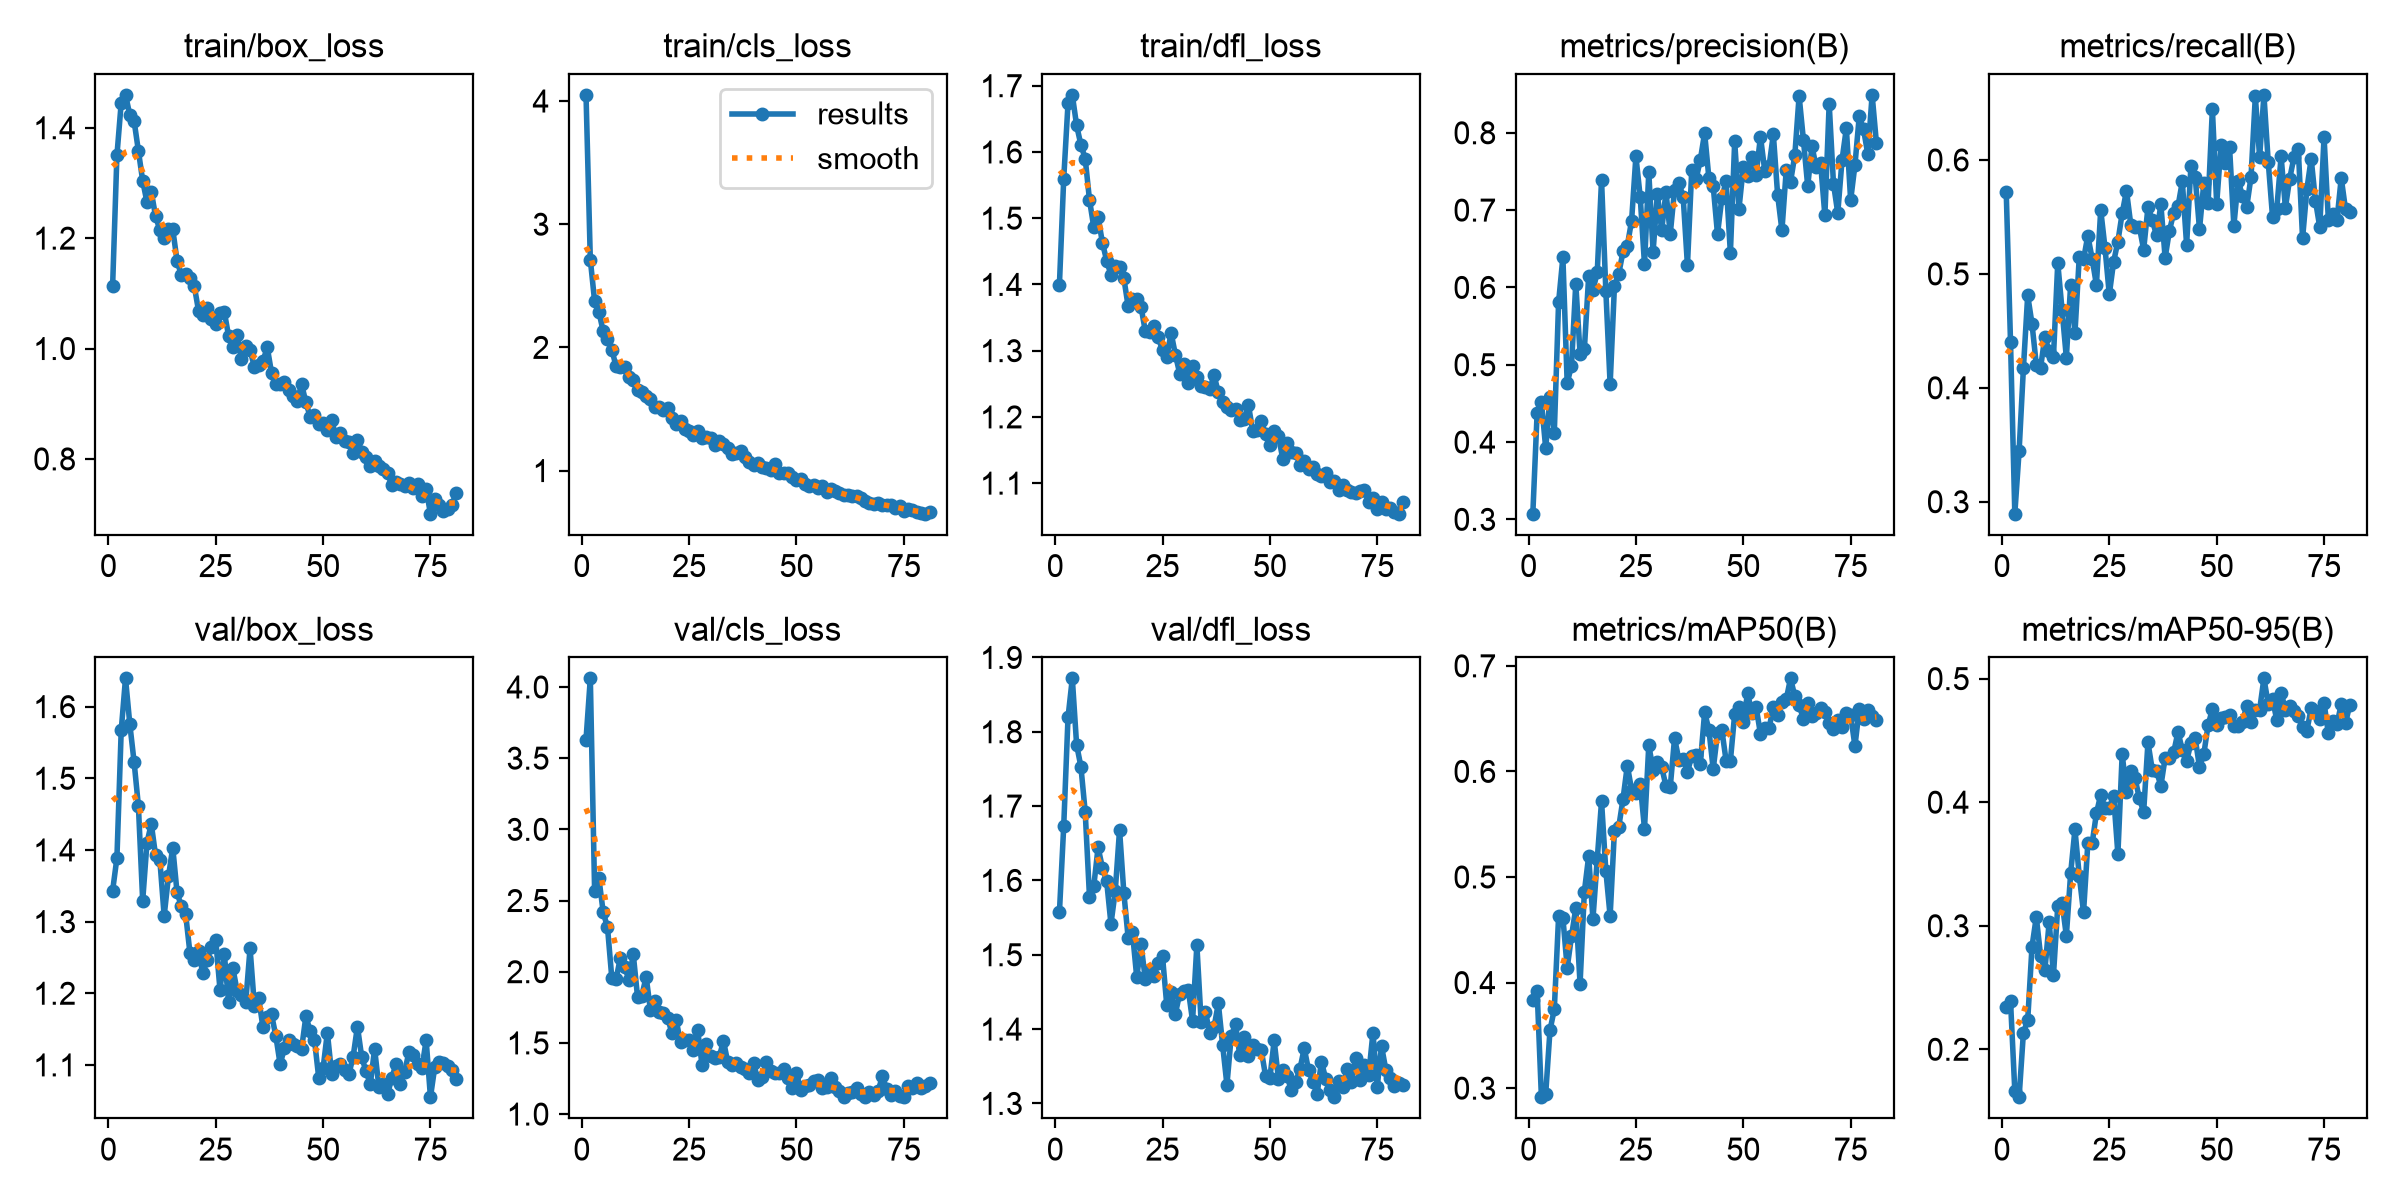
\includegraphics[width=0.96\textwidth]{results/validation_best/results.png}
\caption{Training and validation curves of the YOLO11n model.}
\label{fig:curves}
\end{figure*}

Epoch 61 achieved the highest recorded mAP50 and mAP50-95. The deployment program filters the checkpoint output by class name and retains bottle, mouse, and laptop detections required by this experiment.

\begin{figure}[!t]
\centering
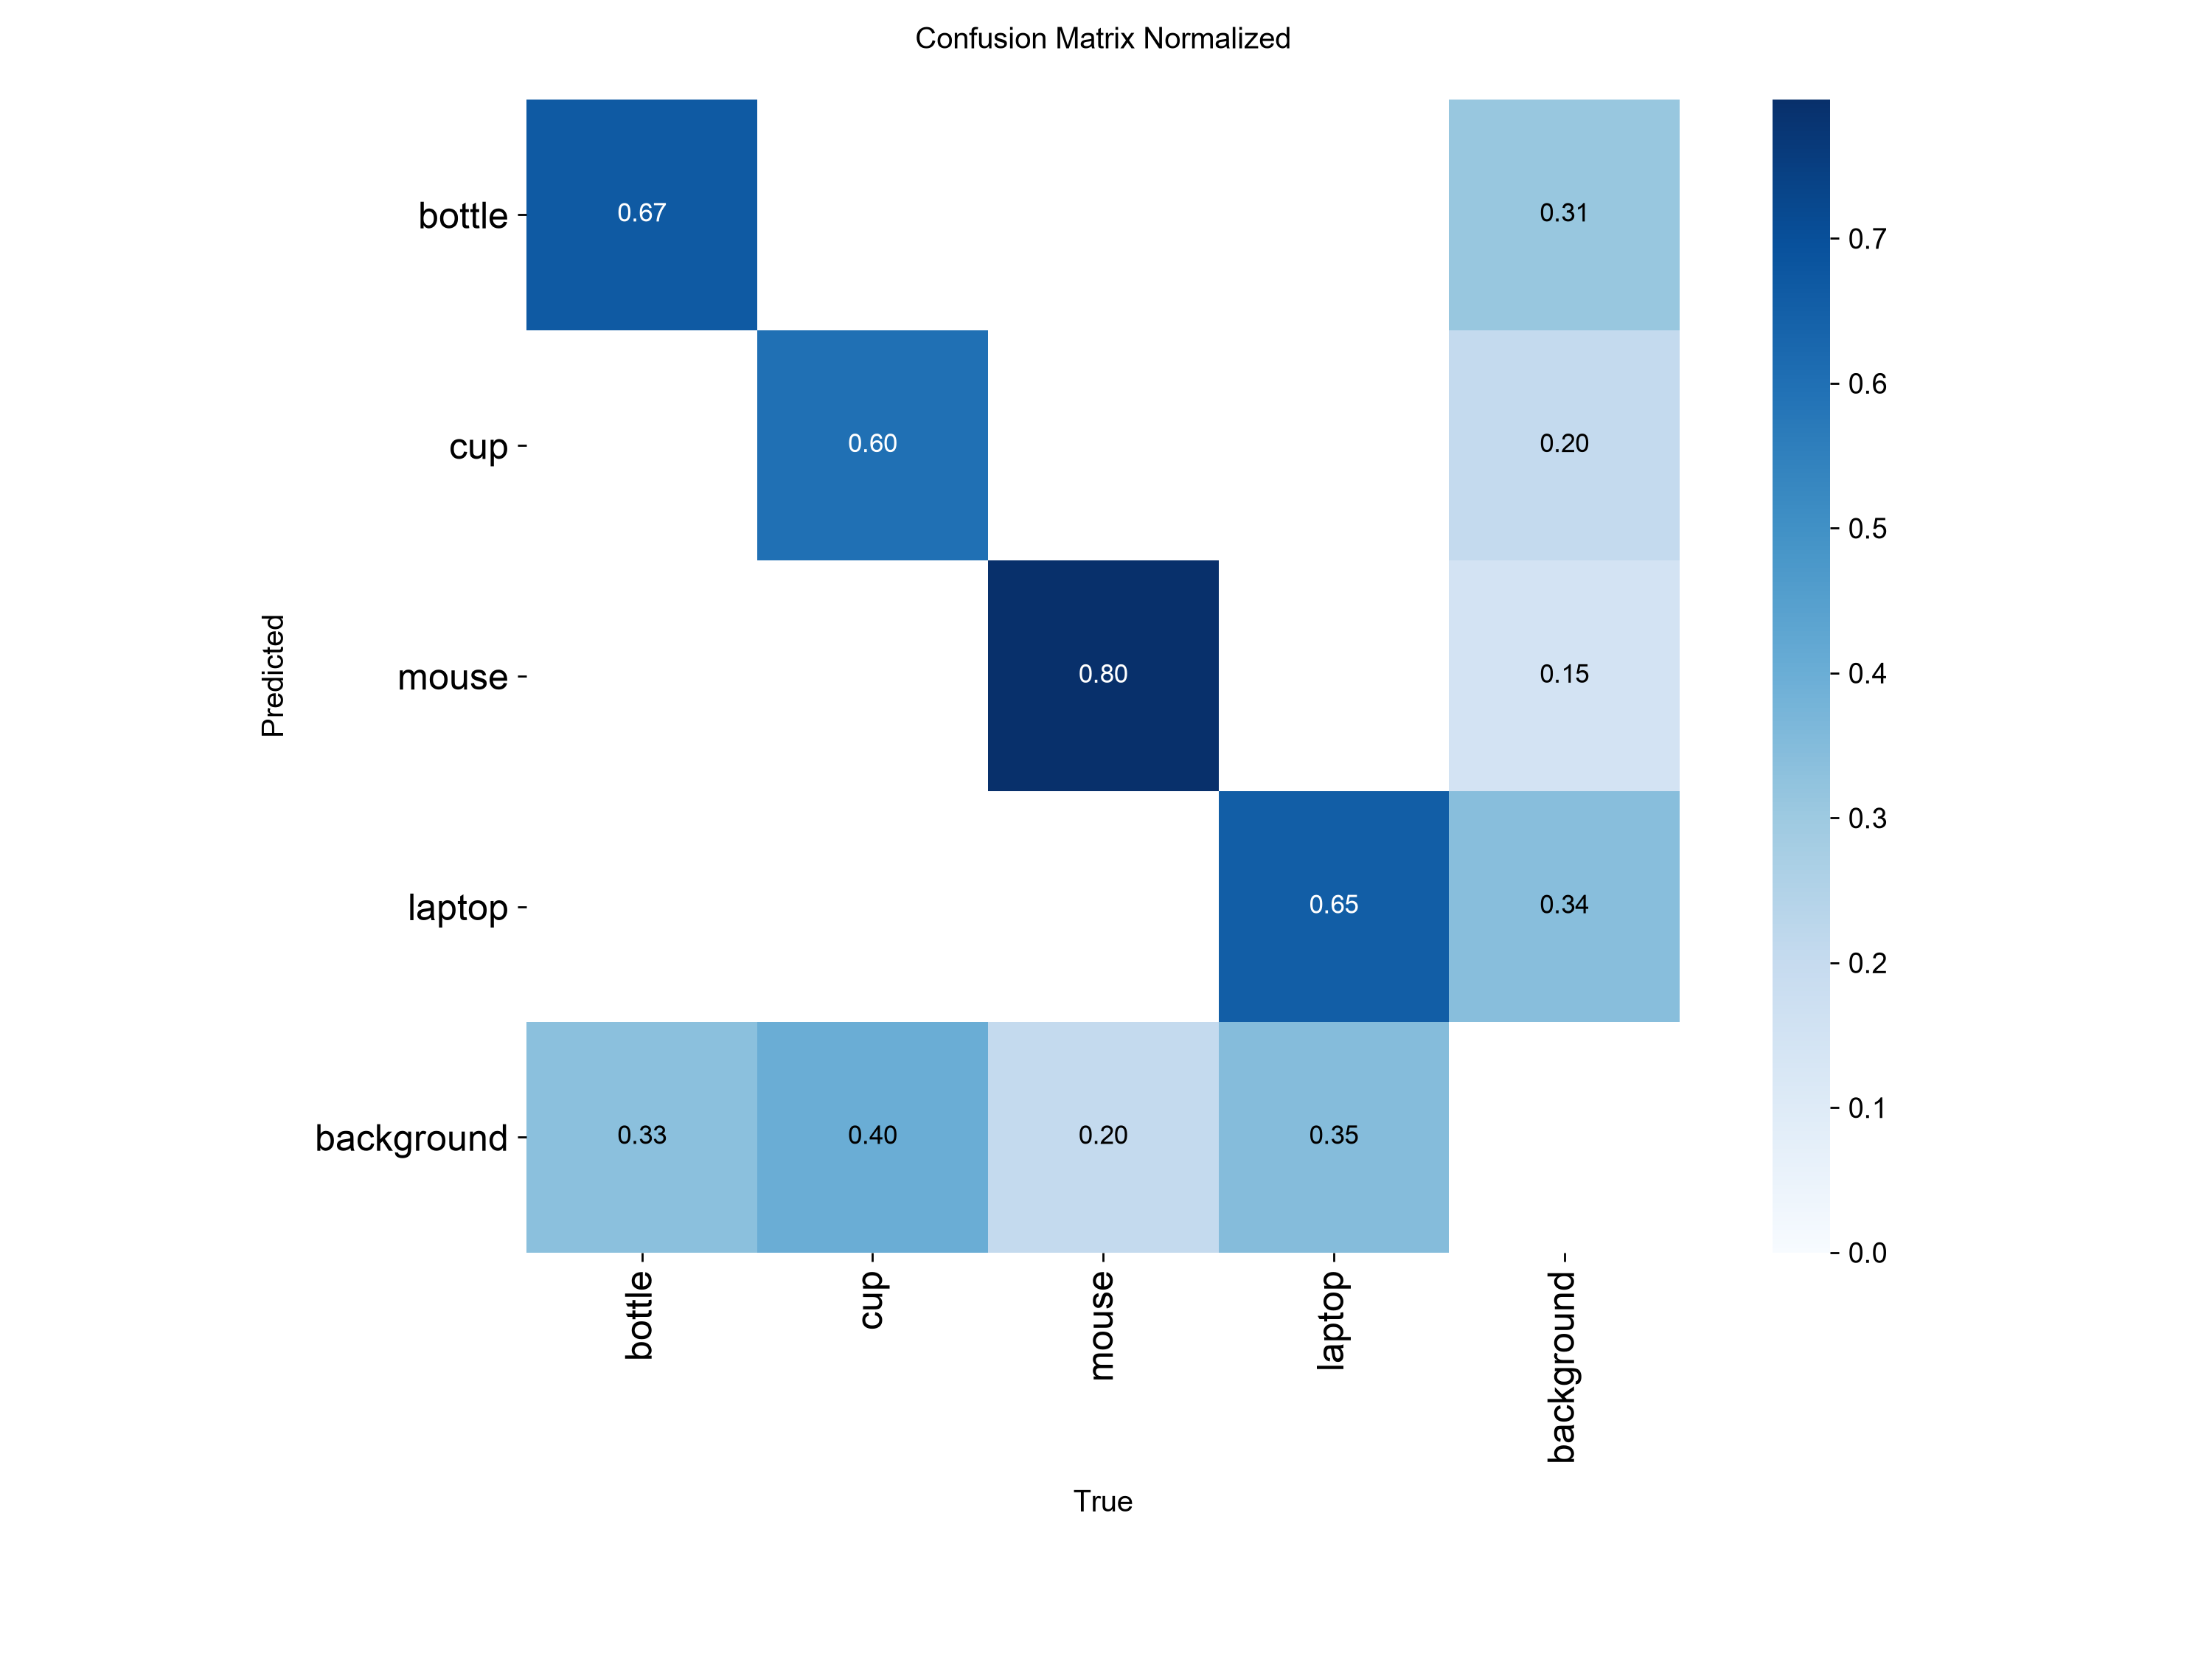
\includegraphics[width=0.98\columnwidth]{results/validation_best/confusion_matrix_normalized.png}
\caption{Normalized confusion matrix of the trained model.}
\label{fig:confusion}
\end{figure}

\section{Experimental Procedure and Implementation}

\subsection{Data Organization and Annotation Validation}
The collected images were first divided into training and validation sets. Each image was paired with a YOLO label file of the same base name. Every annotation contains a class index, normalized center coordinates, and normalized bounding-box width and height. The script \path{scripts/check_dataset.py} was used to verify image-label pairing, field counts, valid class indices, and coordinate ranges. After validation, the generated statistics confirmed 734 training images, 159 validation images, 893 images in total, and 1,483 annotated objects.

\subsection{YOLO11n Training and Weight Selection}
Transfer learning was performed from a pretrained YOLO11n model on the Mac MPS device. The run used a 640-pixel input, batch size 8, seed 42, a maximum of 100 epochs, and early-stopping patience of 20. Box loss, classification loss, DFL loss, precision, recall, mAP50, and mAP50-95 were recorded at every epoch. After training ended at epoch 81, the validation metrics of all checkpoints were compared. Epoch 61 produced the best mAP50 and mAP50-95 and was therefore selected for deployment as \path{models/best.pt}. The file size, class names, and SHA-256 digest were also recorded so that the uploaded Jetson copy could be verified.

\begin{lstlisting}
python3 scripts/check_dataset.py \
  --data data/person1.yaml
python3 scripts/train.py \
  --model yolo11n.pt \
  --data data/person1.yaml \
  --epochs 100 --imgsz 640 \
  --batch 8 --device mps
\end{lstlisting}

\subsection{Jetson Deployment and Camera Inference}
The model, scripts, ROS 2 workspace, and run entry points were copied to \path{/home/nvidia/bht} on the Jetson. Before inference, Python imports for OpenCV, PyTorch, and Ultralytics were checked, and camera index 0 was verified. The \path{run_camera.sh} script locates the project root and \path{models/best.pt}, configures a 640-pixel input, confidence threshold of 0.35, and IoU threshold of 0.45, and selects CUDA when available. The \path{scripts/detect.py} program then reads the camera frame by frame, performs inference, retains bottle, mouse, and laptop, and draws the class, confidence, bounding box, and real-time FPS. Pressing \texttt{q} terminates the run.

Each run creates a timestamped result directory containing \path{annotated.mp4}, the per-object log \path{detections.csv}, and the run summary \path{summary.json}. The program can also save frames at a fixed interval. When at least two classes are present in the same frame, \path{simultaneous_two_classes.jpg} is saved as evidence of simultaneous recognition.

\subsection{ROS 2 Build and Result Publishing}
The ROS 2 experiment uses Humble. The \path{run_ros2.sh} script first sources the system ROS 2 environment, builds the \path{desktop_object_detector} package in \path{ros2_ws} with colcon, and sources the install space. The result-logging node is started before the detector node so that initial messages are not lost. The detector uses the same model, camera, and thresholds as the stand-alone program. It publishes each frame's detections as a JSON string on \path{/desktop_detector/detections} and real-time frame rate as a Float32 message on \path{/desktop_detector/fps}. The logging node subscribes to the detection topic, writes one message per line to \path{detections.jsonl}, and summarizes the message count, box count, and per-class count at shutdown.

\begin{lstlisting}
cd /home/nvidia/bht
/bin/bash run_camera.sh 0
/bin/bash run_ros2.sh 0
\end{lstlisting}

\subsection{Result Organization and Acceptance Test}
After each run, \path{summary.json} and the detection logs were read to obtain the total frame count, duration, mean FPS, number of boxes, and per-class counts. Twenty different camera scenes were then selected for manual review. Each scene was judged by comparing the detected class with the physical object, and the overall accuracy was calculated. Only four representative images are included in the report; the remaining cases are retained in \path{20example/}. The final check covered multi-class detection, two classes in the same frame, accuracy of at least 80\%, Jetson speed of at least 5 FPS, ROS 2 publishing, saved videos, and preserved failure cases.

\begin{figure*}[!t]
\centering
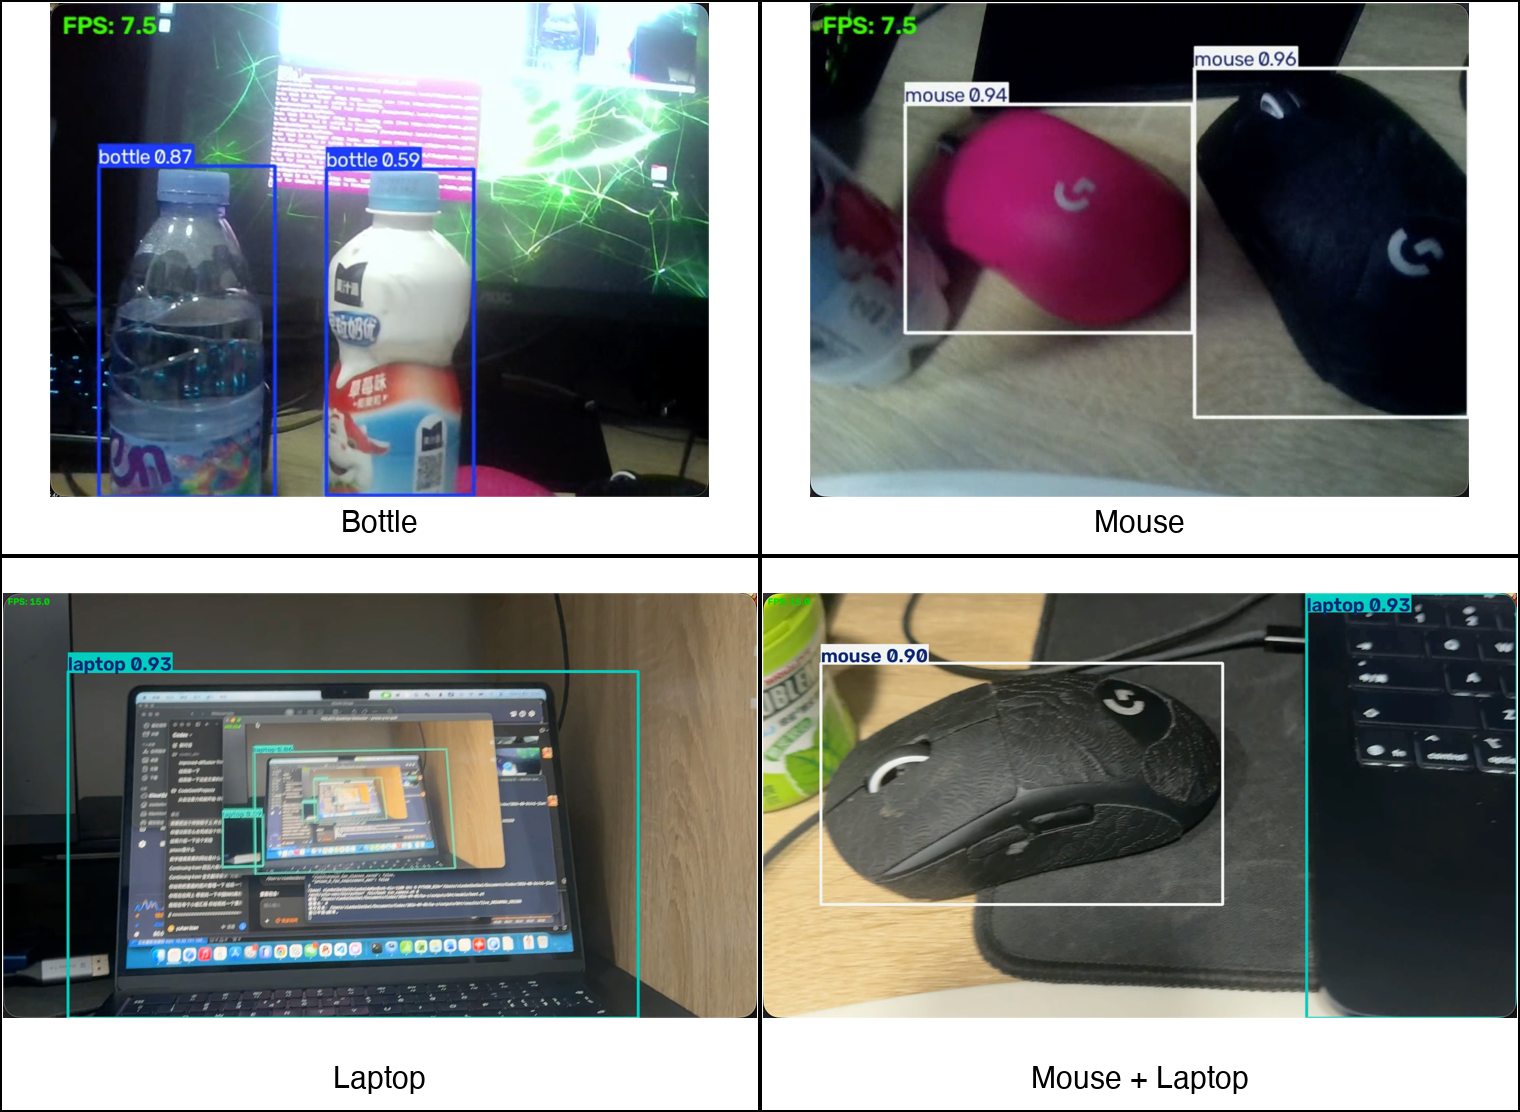
\includegraphics[width=0.86\textwidth]{report_assets/four_cases_color.png}
\caption{Four representative detection results.}
\label{fig:four}
\end{figure*}

\section{Experimental Results}

\subsection{Real-Time Performance}
Table~\ref{tab:runtime} reports three real-time runs. The final three-class Jetson acceptance run processed 411 frames at a mean speed of 7.092 FPS, exceeding the 5 FPS requirement. The long Jetson run processed 30,714 frames at 11.370 FPS. The macOS run was retained as a local reproduction baseline.

\begin{table}[!t]
\caption{Real-Time Runtime Results}
\label{tab:runtime}
\centering
\footnotesize
\begin{tabular}{lrrrr}
\toprule
Run & Frames & Time (s) & Mean FPS & Boxes \\
\midrule
Jetson long & 30,714 & 2,701.302 & 11.370 & 9,760 \\
Jetson final & 411 & 57.956 & \textbf{7.092} & 790 \\
macOS baseline & 1,390 & 94.048 & 14.780 & 1,400 \\
\bottomrule
\end{tabular}
\end{table}

\subsection{Twenty-Case Evaluation}
The \path{20example/} directory contains 20 acceptance-test screenshots. Manual review found 20 correct cases and no incorrect cases, giving an accuracy of 100\%, above the required 80\%. Four representative scenes showing bottle, mouse, laptop, and simultaneous mouse and laptop detection are presented in Fig.~\ref{fig:four}; the other 16 images remain in the submission directory.

\subsection{ROS 2 Results}
The ROS 2 run saved 376 detection messages. Targets were present in 363 frames, with 751 bounding boxes in total. The detailed statistics are listed in Table~\ref{tab:ros}.

\begin{table}[!t]
\caption{ROS 2 Result Statistics}
\label{tab:ros}
\centering
\footnotesize
\begin{tabular}{lr}
\toprule
Metric & Value \\
\midrule
Published and saved messages & 376 \\
Frames containing detections & 363 \\
Detected-frame ratio & 96.54\% \\
Total bounding boxes & 751 \\
bottle / mouse / laptop & 243 / 440 / 68 \\
Mean nonzero FPS & 7.148 \\
\bottomrule
\end{tabular}
\end{table}

\begin{figure*}[!t]
\centering
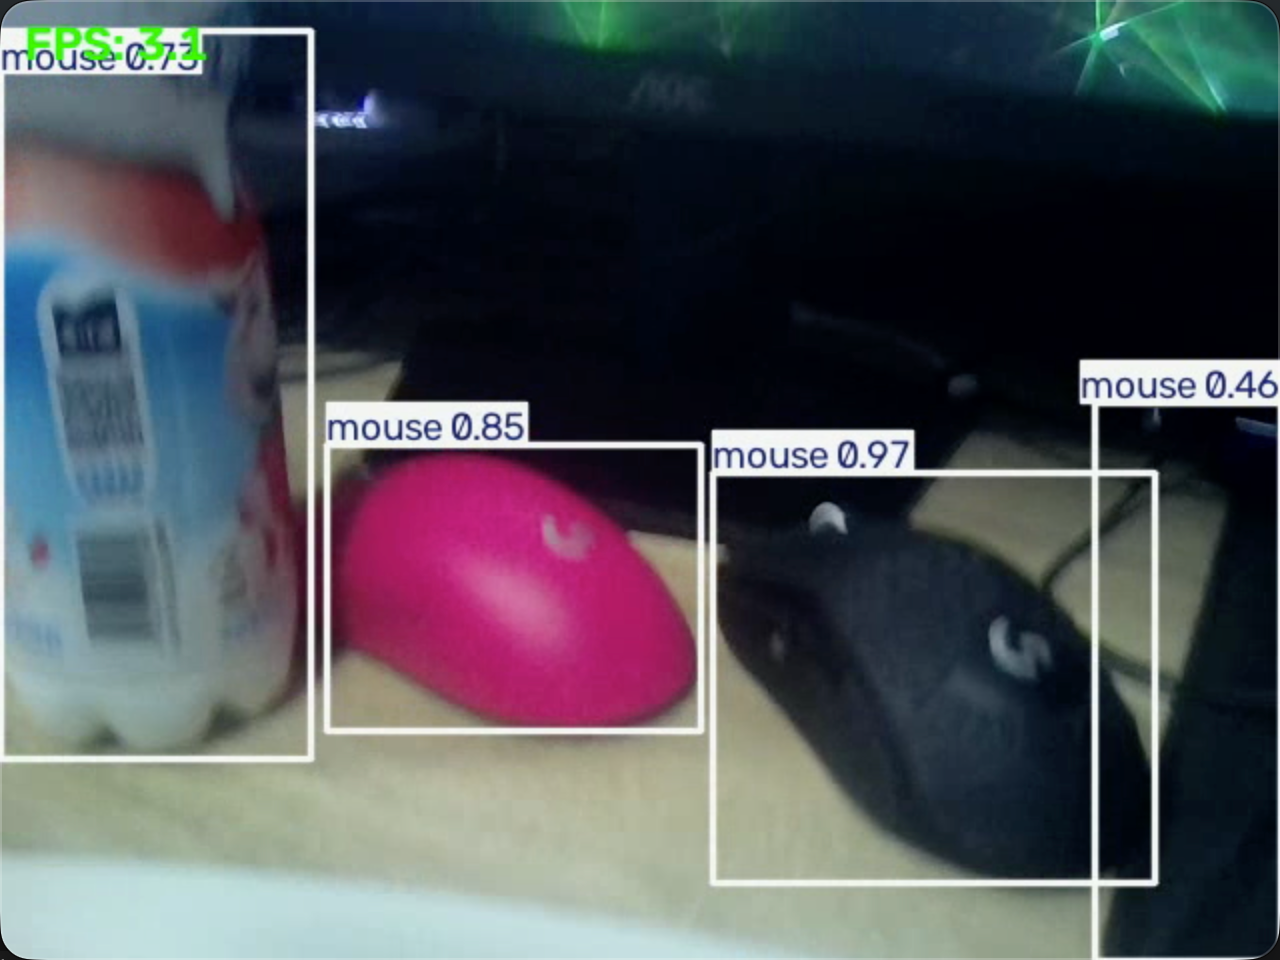
\includegraphics[width=0.48\textwidth]{error_work/0684989f21b5b3b1a189b8508dde6f61.png}\hfill
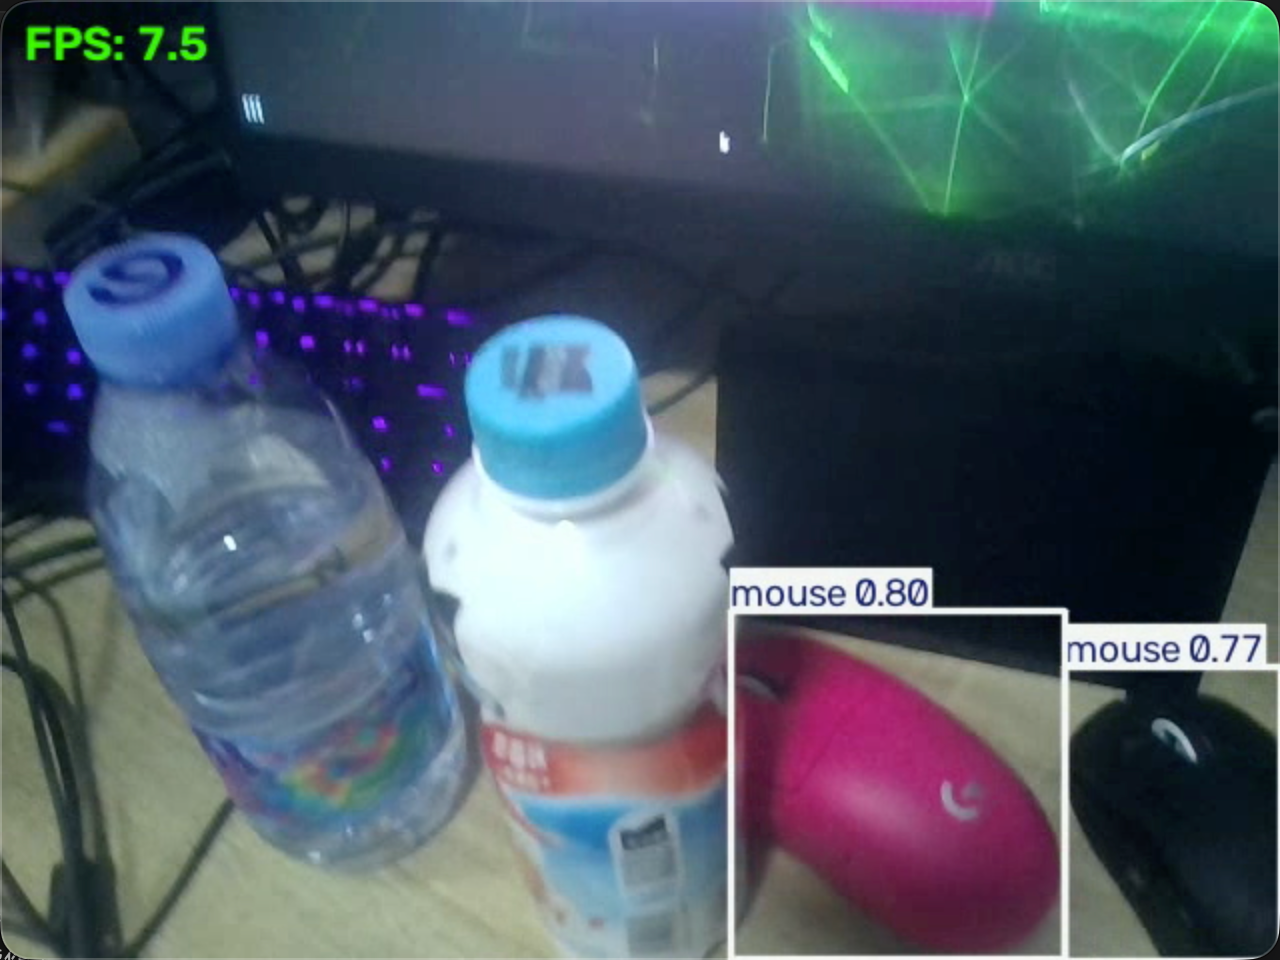
\includegraphics[width=0.48\textwidth]{error_work/413e8f8a8a17942f6556ffee22c426b3.png}
\caption{Typical failure cases. Left: a blurred, edge-truncated bottle is classified as mouse. Right: both mice are detected correctly, while both bottles are missed.}
\label{fig:errors}
\end{figure*}

\subsection{Result Analysis}
The training curves show that box loss, classification loss, and DFL loss decreased rapidly during the first 20 epochs and then converged gradually. Validation mAP50 and mAP50-95 reached a plateau after approximately 60 epochs. Although epoch 80 produced the highest precision, its recall and aggregate mAP values were lower than those of epoch 61, indicating that selecting a checkpoint solely by precision would increase the risk of missed detections. Epoch 61, which maximized both mAP50 and mAP50-95, was therefore used for deployment because it provides a better precision-recall balance for continuous camera inference.

The normalized confusion matrix gives diagonal values of 0.67, 0.80, and 0.85 for bottle, mouse, and laptop, respectively. Classification of laptop and mouse is comparatively stable, whereas bottle is more sensitive to background clutter, occlusion, and motion blur. The class counts, object scales, and camera-distance distributions are not fully balanced across the dataset, which helps explain the observed bottle misclassification and missed detections.

Both Jetson runs exceeded 5 FPS. The long run reached 11.370 FPS, whereas the final acceptance run reached 7.092 FPS. The difference is mainly attributable to the number of visible targets and the additional overhead of rendering, video writing, and screenshot saving. The ROS 2 run recorded 376 messages, 363 of which contained targets, for a detected-frame ratio of 96.54\%. A total of 751 boxes were published with class, confidence, coordinates, and frame-rate information. These results show that the detector and logger operated reliably together and supported both live display and experiment reproduction.

\subsection{Analysis of Typical Failure Cases}
In the left image of Fig.~\ref{fig:errors}, only part of the bottle is visible at the left edge of the frame, and the object is affected by motion blur and truncation. The model assigns it to mouse with a confidence of 0.71, which is a class error. In the same frame, the red and black mice are correctly detected with confidences of 0.85 and 0.97. The bottle label, shadow, and blurred outline create local textures similar to a mouse, while the complete bottle neck and body contour are absent. The model therefore lacks the global shape evidence needed to identify the object as bottle.

In the right image of Fig.~\ref{fig:errors}, the two mice are correctly detected with confidences of 0.80 and 0.77, but the transparent bottle and the white beverage bottle do not receive bottle boxes, which constitutes two missed detections. Reflections on the transparent material, low contrast between the white bottle and the bright display background, and close spacing among objects may have reduced the bottle candidate confidence below the 0.35 threshold. This case shows that mouse recognition remains stable in a normal desktop scene, whereas bottle detection is less robust under reflection, low contrast, and partial occlusion.

These errors can be reduced by adding edge-truncated, motion-blurred, backlit, transparent-bottle, and multi-object occlusion examples to the training set and by checking the annotation completeness of small and truncated objects. Brightness, blur, and crop augmentation can also be strengthened. During deployment, class-specific confidence thresholds should be compared on the validation set. A modestly lower bottle threshold may improve recall, but false positives must be monitored so that recall is not increased at the expense of unacceptable misclassification.

\balance
\section{Submission Package}

The experiment is organized as a GitHub repository. Table~\ref{tab:files} lists the submitted contents.

\begin{table}[H]
\caption{GitHub Repository Contents}
\label{tab:files}
\centering
\footnotesize
\begin{tabularx}{\columnwidth}{>{\ttfamily}p{0.34\columnwidth}X}
\toprule
Folder/file & Contents \\
\midrule
data/, dataset/ & Configuration, images, and YOLO labels \\
models/ & best.pt and model metadata \\
scripts/ & Training, validation, inference, and evaluation \\
ros2\_ws/src/ & ROS 2 package source code \\
results/ & Validation data, video, CSV, JSON, and JSONL \\
20example/ & Twenty acceptance-test images \\
error\_work/ & Representative failure cases \\
run\_camera.sh & Camera inference entry point \\
run\_ros2.sh & ROS 2 execution entry point \\
bht\_ieee\_report.* & LaTeX source and PDF report \\
\bottomrule
\end{tabularx}
\end{table}

\section{Conclusion}

This experiment completed custom dataset preparation, YOLO11n training, real-time Jetson camera inference, and ROS 2 result publishing. The system detects bottle, mouse, and laptop, supports simultaneous recognition of two classes, achieved 100\% accuracy in the 20-case manual evaluation, and reached 7.092 FPS in the final Jetson acceptance run. It also saved annotated video, structured logs, and representative failure cases. The results satisfy the assignment requirements, and the engineering artifacts have been organized for GitHub submission.

\end{document}
